
\def\anon{1} %% set to 1 for anonymous submissions, hides acknowledgements and author names
\def\full{1} %% set to 0 for springer proceedings


\ifnum\full=1
\documentclass[11pt]{llncs}


\addtolength{\parskip}{1pt}
\else
\documentclass[10pt, runningheads]{llncs}
\usepackage{times}

\fi




\usepackage{makeidx}
\usepackage[dvips]{graphicx}
\usepackage{graphicx}

\usepackage{comment}

\usepackage{listings}
\usepackage[mathscr]{eucal}
\usepackage{bm}
\usepackage{array}
\usepackage{url}
\usepackage{calc}
\usepackage{float}
\usepackage{latexsym}
\usepackage{rotating}
\DeclareGraphicsExtensions{.eps,.jpg,.png,.pdf}
%\usepackage[usenames, dvipsnames]{xcolor}
\usepackage[dvipsnames]{xcolor}
\usepackage[sort,nocompress]{cite}
\usepackage{colortbl}
\usepackage{multirow}
\usepackage{lscape}
\usepackage{amsmath}
\let\proof\relax
\let\endproof\relax
\usepackage{amsthm,amsfonts,amssymb}
\usepackage{hyperref}
\usepackage{pdflscape}


%\usepackage{natbib}

\def\rmdefault{ptm}

\usepackage{setspace}
\usepackage{color}
\ifnum\full=1
\usepackage[margin=0.9in]{geometry}
\usepackage{fullpage}

\setlength{\parskip}{0cm}

%\setstretch{1.03}
%\addtolength{\parskip}{1pt}
\setcounter{page}{0}
\renewcommand{\tabcolsep}{5pt}
\else
\renewcommand{\tabcolsep}{0pt}
\fi

\renewcommand{\arraystretch}{1.2}

\hyphenpenalty=5000
\tolerance=1000




%\ifnum\full=1
%\usepackage{natbib}
%\bibliographystyle{alpha}
%\setlength{\bibsep}{0pt}
%\renewcommand{\bibsection}{\section*{References}\small}
%\else
%\usepackage[numbers]{natbib}
%\bibliographystyle{splncs04}
%\fi



\DeclareMathOperator{\Exp}{E}
\DeclareMathOperator{\Var}{Var}
\DeclareMathOperator{\poly}{poly}
\DeclareMathOperator{\Supp}{Supp}

\usepackage{enumitem}


\usepackage{tikz}
\usetikzlibrary{arrows,shapes}
\usetikzlibrary{plotmarks}


%notes

%\definecolor{myorange}{rgb}{0.99,0.6,0.25}
%\newcommand{\pmnote}[1]{\colorbox{myorange}{\parbox{0.9\linewidth}{[{\footnotesize {\bf PM:} { {#1}}}]}}}


\definecolor{mycolor}{rgb}{0.75,0.95,0.05}
\newcommand{\pmnote}[1]{\colorbox{mycolor}{\parbox{0.9\linewidth}{[{\footnotesize {\bf PM:} { {#1}}}]}}}

\newcommand{\tsnote}[1]{\colorbox{orange}{\footnotesize\color{white}\textbf{TS: }#1}}

\definecolor{unmellowyellow}{rgb}{1.0, 1.0, 0.4}
\newcommand{\agnote}[1]{\colorbox{unmellowyellow}{\parbox{0.9\linewidth}{[{\footnotesize {\bf AG:} { {#1}}}]}}}
%% Sets

\newcommand{\Z}{\mathbb{Z}}
\newcommand{\N}{\mathbb{N}}
\newcommand{\R}{\mathbb{R}}
\newcommand{\C}{\mathbb{C}}
\newcommand{\F}{\mathbb{F}}
\newcommand{\Znm}{\mathbb{Z}_q^{n \times m}}

%matrices
\newcommand{\matzero}{\mathbf{0}}
\newcommand{\matA}{\mathbf{A}}
\newcommand{\matB}{\mathbf{B}}
\newcommand{\matC}{\mathbf{C}}
\newcommand{\matE}{\mathbf{E}}
\newcommand{\matF}{\mathbf{F}}
\newcommand{\matG}{\mathbf{G}}
\newcommand{\matI}{\mathbf{I}}
\newcommand{\matM}{\mathbf{M}}
\newcommand{\matP}{\mathbf{P}}
\newcommand{\matR}{\mathbf{R}}
\newcommand{\matS}{\mathbf{S}}
\newcommand{\matT}{\mathbf{T}}
\newcommand{\matU}{\mathbf{U}}
\newcommand{\matV}{\mathbf{V}}
\newcommand{\matW}{\mathbf{W}}
\newcommand{\matX}{\mathbf{X}}
\newcommand{\matY}{\mathbf{Y}}
\newcommand{\matZ}{\mathbf{Z}}


%vectors
\newcommand{\veca}{\mathbf{a}}
\newcommand{\vecb}{\mathbf{b}}
\newcommand{\vecc}{\mathbf{c}}
\newcommand{\vecd}{\mathbf{d}}
\newcommand{\vece}{\mathbf{e}}
\newcommand{\veci}{\mathbf{i}}
\newcommand{\vecj}{\mathbf{j}}
\newcommand{\veck}{\mathbf{k}}
\newcommand{\vecl}{\mathbf{l}}
\newcommand{\vecm}{\mathbf{m}}
\newcommand{\vecp}{\mathbf{p}}
\newcommand{\vecr}{\mathbf{r}}
\newcommand{\vecs}{\mathbf{s}}
\newcommand{\vecv}{\mathbf{v}}
\newcommand{\vecw}{\mathbf{w}}
\newcommand{\vecu}{\mathbf{u}}
\newcommand{\vecx}{\mathbf{x}}
\newcommand{\vecy}{\mathbf{y}}
\newcommand{\vecz}{\mathbf{z}}





%FiLIP notations

\newcommand{\FLIP}{\textsf{FLIP}}
\newcommand{\IFPl}{\text{Improved Filter Permutator} }
\newcommand{\IFPs}{\text{IFP} }

\newcommand{\FiLIP}{\textsf{FiLIP}}
\newcommand{\FiLIPDSM}{\mathsf{FiLIP}_{\mathsf{DSM}}}
\newcommand{\FiLIPXMAJ}{\mathsf{FiLIP}_{\mathsf{XMAJ}}}

%Boolean functions

\newcommand{\Bfn}[1]{\mathcal{B}_{#1}}
\newcommand{\BN}{\mathcal{B}_n}
\newcommand{\Bn}[1]{\mathcal{B}_{#1}}
\newcommand{\Bnstar}[1]{\mathcal{B}_{#1}^*}

\newcommand{\Bvad}[3]{\mathcal{B}({#1},{#2},{#3})}


\newcommand{\AI}{\mathsf{AI}}
\newcommand{\AN}{\mathsf{AN}}
%\newcommand{\difAN}[1]{\Delta_{\mathsf{AN}}(#1)}
%\newcommand{\DAN}{\mathsf{d}\mathsf{AN}}
%\newcommand{\Sd}{\mathsf{S}_\mathsf{d}}
\newcommand{\SD}{\mathsf{SD}}
\newcommand{\FAI}{\mathsf{FAI}}
\newcommand{\NL}{\mathsf{NL}}
\newcommand{\NLk}[1]{\mathsf{NL}_{#1}}
%\newcommand{\NLd}{\mathsf{NL_d}}
\newcommand{\res}{\mathsf{res}}
\newcommand{\bal}{\mathsf{bal}}
\newcommand{\gnlk}{\mathsf{GWNL}}


\newcommand{\DS}[1]{\mathsf{DS}(#1)}
\newcommand{\DSR}[2]{\mathsf{DS}^{#2}(#1)}
%\newcommand{\matAI}[3]{\mathbf{A}_{#2,#3}(#1)}

\newcommand{\WPB}[1]{\mathcal{WPB}_{#1}}
\newcommand{\WAPB}[1]{\mathcal{WAPB}_{#1}}
\newcommand{\SWAPB}[1]{\mathcal{SWAPB}_{#1}}
\newcommand{\SYM}[1]{\mathcal{SYM}_{#1}}
%for affine weightwise: degree and number of variables
\newcommand{\WD}[2]{\mathcal{WD}^{#1}_{#2}}
\newcommand{\Ekn}[2]{\mathsf{E}_{#1,#2}}
\newcommand{\Code}[2]{\mathsf{P}_{#1,#2}}
\newcommand{\mdist}[2]{\mathsf{d}_{#1,#2}}
%\newcommand{\Dka}[2]{\mathsf{D}_{#1}(#2)}
\newcommand{\Dnka}[3]{\mathsf{D}_{#1,#2}(#3)}

\newcommand{\dis}{\mathsf{c_1}}




\newcommand{\mnlk}[2]{\mu_{#1,#2}}
\newcommand{\Mnlk}[2]{\mathsf{M}_{#1,#2}}
\newcommand{\mnl}[1]{\mu_{#1}}
\newcommand{\Mnl}[1]{\mathsf{M}_{#1}}

\newcommand{\DistWkn}[2]{\mathfrak{W}_{#1,#2}}
\newcommand{\DistWn}[1]{\mathfrak{W}_{#1}}
\newcommand{\Dkn}[2]{\mathfrak{D}_{#1,#2}}
\newcommand{\Dn}[1]{\mathfrak{D}_{#1}}

\newcommand{\kraw}[3]{\mathsf{K}_{#1}(#2,#3)}
\newcommand{\phikn}[2]{\varphi_{#1,#2}}

\newcommand{\const}[2]{g_{#1,#2}}
\newcommand{\setn}[1]{S_{#1}}
\newcommand{\symsetsmall}[1]{A_{#1}}
\newcommand{\symset}[2]{B_{#1,#2}}


%usual notations
\newcommand{\supp}{\mathsf{supp}}
\newcommand{\suppk}[1]{\mathsf{supp}_{#1}}
\newcommand{\w}{\mathsf{w_H}}
\newcommand{\hd}{\mathsf{d_H}}
\newcommand{\degg}{\mathsf{deg}}
\newcommand{\Span}{\mathsf{Span}}
\newcommand{\rank}{\mathsf{rank}}
%Walsh transform
\newcommand{\wt}[1]{\mathcal W_{#1}} 
\newcommand{\Wsupp}[1]{\mathsf{Wsupp}_{#1}} 
%restricted Walsh transform W_k,a (f)
\newcommand{\wtk}[2]{\mathcal{W}_{#1,#2}} 

%S-equivalent classes
\newcommand{\sclass}[1]{\mathcal{S}(#1)}


\newcommand{\set}[1]{\left\{#1\right\}}
\newcommand{\mAN}[1]{\mathsf{d}_{#1}}


%gates
\newcommand{\AND}{\textsf{AND}}
\newcommand{\XOR}{\textsf{XOR}}
\newcommand{\MUX}{\textsf{MUX}}


%families of functions
\newcommand{\MAJ}{\textsf{MAJ}}
\newcommand{\DSM}{\textsf{DSM}}
\newcommand{\XORTHR}{\textsf{XOR-THR}}
\newcommand{\XORMAJ}{\textsf{XOR-MAJ}}

\newcommand{\xorlk}[2]{{\mathsf{XOR}}_{#1}  \mathsf{M}_{#2}} 
\newcommand{\xormaj}[2]{{\mathsf{XOR}}_{#1}  \mathsf{MAJ}_{#2}} 
%\newcommand{\xorthr}[3]{{\mathsf{XOR}}_{#1}  \mathsf{T}_{{#2},{#3}}} 
\newcommand{\xorthr}[3]{{\mathsf{XOR}}_{#1}+\mathsf{T}_{{#2},{#3}}}
\newcommand{\tri}[1]{{T}_{#1}}
\newcommand{\thr}[2]{\mathsf{T}_{{#1},{#2}}}
\newcommand{\xor}[1]{\mathsf{XOR}_{#1}}
\newcommand{\maj}[1]{\mathsf{MAJ}_{#1}}


\newcommand{\nbf}[1]{\mathsf{C}_{#1}}
\newcommand{\nbfodd}[2]{\mathsf{A}_{#1,#2}}
\newcommand{\nbfeven}[2]{\mathsf{B}_{#1,#2}}

%direct sum vector and simplified value vector
\newcommand{\dsv}[1]{\mathbf{m}_{#1}}
\newcommand{\svv}[1]{\mathbf{s}_{#1}}

% Define a custom theorem style for bold optional arguments
\newtheoremstyle{boldoptional} % Name of the style
  {3pt}                        % Space above
  {3pt}                        % Space below
  {\itshape}                   % Body font
  {}                           % Indent amount
  {\bfseries}                  % Theorem head font
  {.}                          % Punctuation after theorem head
  { }                          % Space after theorem head
  {\thmname{#1}\thmnumber{ #2}\thmnote{ (\textbf{#3})}} % Bold optional argument

% Apply the new style to Property
\theoremstyle{boldoptional}
\newtheorem{Prop}{Property}
\newtheorem{Cons}{Construction}


% For algorithms
\usepackage{algorithm,algpseudocode}

\renewcommand{\algorithmicrequire}{\textbf{Input:}}
\renewcommand{\algorithmicensure}{\textbf{Output:}}
% \renewcommand{\ALG@name}{Construction}
\newenvironment{constr}[1][htb]{%
\floatname{algorithm}{Construction}% Update algorithm name
   \begin{algorithm}[#1]%
  }{\end{algorithm}}
 
\algnewcommand\algorithmicparfor{\textbf{par-for}}
\algdef{S}[FOR]{ParFor}[1]{\algorithmicparfor\ #1\ \algorithmicdo}
 
%latin

\newcommand{\ie}{\textit{i.e.}}
\newcommand{\eg}{\textit{e.g.}}
\newcommand{\ea}{\textit{et al.}}

%Tim's stuff
\newtheorem{Corollary}{Corollary}
\newcommand{\ii}{\mathrm i\mkern1mu} %Imaginary unit
\newcommand{\ee}{\mathrm e\mkern1mu} %Euler constant
\newcommand{\dd}{\,\mathrm d} %Differential
\newcommand{\ui}[1]{^{(#1)}} %Upper index
\newcommand{\mycomment}[1]{} %Comment out entire parts
\usepackage{mleftright}
\mleftright %Less space when using \left and \right


\newcommand{\tablecaption}[1]{%
   \vspace{3pt} % Adds space above the caption
   \caption{#1} % Displays the caption text
}

\let\leq=\leqslant %Replace symbol for \leq
\let\geq=\geqslant %Replace symbol for \geq

\newcommand{\hwbf}{\textsf{HWBF}}

%No line break before lists
\makeatletter
\@beginparpenalty=10000
\makeatother


\begin{document}
	\title{Draft: Notes on the revised Hidden weight function}

	
	\titlerunning{Notes on the revised Hidden weight function}
	\author{
%		\mbox{Pierrick M\'eaux}\inst{1}
	}
	
	\authorrunning{ P. M\'eaux}
	
	\institute{
	Luxembourg university, Luxembourg\\
%		\email{pierrick.meaux@uni.lu}		
	}
	

	
	
	
	%----------------------------------------------------------------
	\maketitle


\institute{
	University of Luxembourg, Luxembourg\\
	\email{pierrick.meaux@uni.lu}		
}	
	
	\begin{abstract}
	
		
	\end{abstract}


\section{Introduction}

\section{Preliminaries}


\subsection{Boolean functions and weightwise considerations}

In this part we recall general concepts on Boolean functions and their weightwise properties we use in this article. 
For a deeper introduction on Boolean functions and their cryptographic parameters we refer to the survey of \eg~\cite{Carlet20} and to~\cite{TOSC:CarMeaRot17} for the weightwise properties, also called properties on the slices.
For $k \in [0,n]$ we denote $\Ekn{k}{n}$ the set $\{x\in \F_2^n \, | \, \w(x)=k  \}$ and call it slice of the Boolean hypercube (of dimension $n$). 
Accordingly, the Boolean hypercube is partitioned into $n+1$ slices where the elements have the same Hamming weight.

\begin{definition}[Boolean Function]\label{def:bool_f}
	A Boolean function $f$ in $n$ variables is a function from $\F_2^n$ to $\F_2$. 
	The set of all Boolean functions in $n$ variables is denoted by $\BN$, and we denote $\BN^*$ the set without the null function.
\end{definition}


To denote when a property or a definition is restricted to a slice we use the subscript $k$. 
For example, for a $n$-variable Boolean function $f$ we denote its support $\supp(f)=\{x\in \F_2^n \, | \, f(x)=1  \}$ and we denote $\suppk{k}(f)$ its support restricted to a slice, that is $\supp(f)\cap \Ekn{k}{n}$.


\begin{definition}[Balancedness]\label{def:balancedness}
	A Boolean function $f\in \BN$ is called balanced if $|\supp(f)|=2^{n-1}=|\supp(f+1)|$. 
	
	For $k\in [0,n]$ the function is said balanced on the slice $k$ if $||\suppk{k}(f)|-|\suppk{k}(f+1)| |\le 1$. In particular when $|\Ekn{k}{n}|$ is even $|\suppk{k}(f)|=|\suppk{k}(f+1)|=|\Ekn{k}{n}|/2$.
\end{definition}

\begin{definition}[Algebraic Normal Form (ANF) and degree]\label{def:anf}
	We call Algebraic Normal Form of a Boolean function $f$ its $n$-variable polynomial representation over $\F_2$ (\textit{i.e.} belonging to $\F_2[x_1,\dots,x_n]/(x_1^2+x_1,\dots,x_n^2+x_n)$):
	\[f(x_1,\dots,x_n)= \sum_{I \subseteq [1,n]} a_I \left( \prod_{i \in I} x_i \right) \]%x_1,\dots,x_n=\sum_{I \subseteq [1,n]} a_I x^I,\]
	where $a_I\in \F_2$. 	
	The (algebraic) degree of $f$, denoted $\degg(f)$ is: \[\degg(f)=\
	\max_{I\subseteq [1,n]}\{ |I|\, | \, a_I=1\}  \text{ if $f$ is not null},0  \text{ otherwise}.\]
\end{definition}




\begin{definition}[Walsh transform and restricted Walsh transform]\label{def:walsh_transform}
	Let $f\in \Bn{n}$ be a Boolean function, its Walsh transform $\wt{f}$ at $a \in \F_2^n$ is defined as:
	\[  \wt{f} (a) := \sum_{x \in \F_2^n} (-1)^{f(x) +  a \cdot x }.\]
	%	The Walsh support is the set $\Wsupp{f}:=\{ a\in \F_2^n\, | \, \wt{f} (a) \neq 0 \}$.
	Let $f\in \Bn{n}$, $S \subset \F_2^n$, its Walsh transform restricted to $S$ at $a \in \F_2^n$ is defined as:
	\[  \wt{f,S} (a) := \sum_{x\in S} (-1)^{f(x)+ax}.\]
	For $S=\Ekn{k}{n}$ we denote $\wt{f,\Ekn{k}{n}} (a)$ by $\wtk{f}{k}(a)$.%, and for $a= 0_{n}$ we denote $\wtk{f}{k}(a)$ as $\wtk{f}{k}(0)$.
\end{definition}


	


%\begin{definition}[Algebraic Immunity] \label{def:ai}
%	The algebraic immunity of a Boolean function $f\in \Bfn{n}$, denoted as $\AI(f)$, is defined as:
%	\[ \AI(f) = \min_{g \neq 0}\{ \degg(g) \; | \; fg = 0 \; \text{or} \; (f + 1)g = 0 \}{,} \]
%	where $\degg(g)$ is the algebraic degree of $g$.
%	The function $g$ is called an annihilator of $f$ (or $f + 1$). 
%	Additionally we denote $\AN(f) = \min_{g \neq 0}\{ \degg(g) \; | \; fg = 0\}$.
%\end{definition}
\begin{definition}[Nonlinearity and weightwise nonlinearity] \label{def:nl}
	The nonlinearity $\NL(f)$ of a Boolean function $f\in \BN$, where $n$ is a positive integer, is the minimum Hamming distance between $f$ and all the affine functions in $\BN$:
	\[ \NL(f) = \min_{g,\, \degg(g)\leq 1} \{ \hd(f,g) \}{,} \]
	where $g(x)=a\cdot x+\varepsilon$, $a\in \F_2^n, \varepsilon\in \F_2$. 	
	The nonlinearity can also be defined from the Walsh transform:
	\[ \NL(f) = 2^{n-1}- \frac{1}{2} \max_{a\in \F_2^n}{|\wt{f}(a)|}. \]
\end{definition}

\begin{definition}[Algebraic immunity] \label{def:ai}
	The algebraic immunity of a Boolean function $f\in \Bfn{n}$, denoted as $\AI(f)$, is defined as:
	\[ \AI(f) = \min_{g \neq 0}\{ \degg(g) \; | \; fg = 0 \; \text{or} \; (f + 1)g = 0 \}{,} \]
	where $\degg(g)$ is the algebraic degree of $g$.
	The function $g$ is called an annihilator of $f$ (or $f + 1$). 
\end{definition}

\subsection{Symmetric Functions}


The $n$-variable \emph{Boolean symmetric functions} are those that are constant on each slice $\Ekn{k}{n}$ for $k\in [0,n]$. 
This class has been assiduously studied in the context of cryptography, see \eg \cite{IEEE:Carlet04,IEEE:CanVid05,INDO:BraPre05,DM:SarMai07,IEEE:QFLW09,Latin:Meaux19,CCDS:Meaux21,IEEE:CarMea21}.
In this paper we mainly consider two families of symmetric functions, which are both bases of the symmetric functions:

\begin{definition}[Elementary symmetric functions]
Let $i\in [0,n]$, the elementary symmetric function of degree $i$ in $n$ variables, denoted $\sigma_{i,n}$, is the function which ANF contains all monomials of degree $i$ and no monomials of other degrees. 
\end{definition}
\begin{definition}[Slice indicator functions]
 Let $k\in [0,n]$, the indicator function of the slice of weight $k$ is defined as:
 \[\forall  x\in \mathbb{F}_2^{n}, \quad \phikn{k}{n}(x) = 1 \text{ if and only if } \w(x) = k.\]
\end{definition}
We recall that bent functions are those Boolean functions achieving maximal nonlinearity.





\subsection{Krawtchouk polynomials}
We use Krawtchouk polynomials and some of their properties to prove one of our results, we give the necessary preliminaries here and refer to \eg ~\cite{book:MacSlo78} for more details.

\begin{definition}[Krawtchouk Polynomials]\label{def:Kraw}
	The Krawtchouk polynomial of degree $k$, with $0\leq k\leq n$ is given by: $ \displaystyle \kraw{k}{\ell}{n}=\sum_{j=0}^{k} (-1)^j \binom{\ell}{j} \binom{n-\ell}{k-j}$. 
	
	Krawtchouk polynomials are characterized by the generating series: $ \displaystyle (1+z)^{n-x} (1-z)^x=\sum_{k=0}^\infty \kraw{k}{x}{n} z^k$.
\end{definition}





\pmnote{Introduce formally HWBF, and weightwise degree d functions}






\section{Main section}
%\subsection{Restricted Walsh transform of $f$ in a recursive fashion}

We study the function $f$ in an even number of variables $n$ defined as the following:
\[f(x_1,\cdots,x_n)=\left(\sum_{i=1}^{n/2} (x_i+1) x_{i+\frac{n}{2}}\right) + \sum_{k=1}^n \phikn{k}{n} x_k.\]

We study the restricted Walsh transform  of $f$ to bound its nonlinearity.

\begin{align*}
\wtk{f}{k}(a)&=\sum_{x \in \Ekn{k}{n}} (-1)^{f(x)+ax}\\
&=\sum_{x \in \Ekn{k}{n}} (-1)^{x_k + \sum_{i=1}^{n/2} (x_i+1) x_{i+\frac{n}{2}}+ ax}\\
&=\sum_{x \in \Ekn{k}{n}} (-1)^{\sum_{i=1}^{n/2} x_i x_{i+\frac{n}{2}}+ (c)x},
\end{align*}
where $c$ is the $n$-length binary vector such that $c=a+e_k+\sum_{i=n/2+1}^n e_i$ where the $e_i$ denotes the canonical vector with "1" in position $i$.

Accordingly, we can study the restricted Walsh transform of this function by analyzing the one of $\sum_{i=1}^{n/2} x_i x_{i+\frac{n}{2}}$, for all $a$. We introduce the following notations.

\begin{definition}
Let $n\in \N$ be an even number, and $a\in \F_2^n$. We denote $d_n$ the function given by: $d_n(x)=\sum_{i \text{ odd}}^n x_i x_{i+1}$, 
and we denote by $\Dnka{n}{k}{a}$:
\[\Dnka{n}{k}{a}= \sum_{x\in \Ekn{k}{n}} (-1)^{d_n(x) +a x}\]
\end{definition}
The limit case of $n=0$ yields that $\Dnka 0ka=1$ if $k=0$ and $\Dnka 0ka=0$ otherwise.

With these notations we obtain a recursive relation for $\Dnka{n}{k}{a}$, and therefore for $\wtk{f}{k}(a)$, denoting $b=(a_1,\cdots,a_{n-2})$ and $y=(x_1,\cdots,x_{n-2})$, we get for any even $n\geq 2$:

\begin{align*}
\Dnka{n}{k}{a}&=\sum_{x\in \Ekn{k}{n}} (-1)^{d_n(x) +a x}\\
&=\sum_{x\in \Ekn{k}{n-2}} (-1)^{d_{n-2}(y) +b y}+
\sum_{x\in \Ekn{k-1}{n-2}} (-1)^{d_{n-2}(y) +b y + a_{n-1}}\\
&+\sum_{x\in \Ekn{k-1}{n-2}} (-1)^{d_{n-2}(y) +b y + a_{n}}
+\sum_{x\in \Ekn{k-2}{n-2}} (-1)^{d_{n-2}(y) +b y +1 + a_{n-1}+ a_{n}}\\
&=\Dnka{n-2}{k}{b}+\left((-1)^{a_{n-1}} + (-1)^{a_{n}}\right)\Dnka{n-2}{k-1}{b} + (-1)^{1+a_{n-1}+a_n} \Dnka{n-2}{k-2}{b}.
\end{align*}

Then it gives three cases:
\begin{itemize}
	\item if $a_{n-1}=a_n=0$, then $\Dnka{n}{k}{a}=\Dnka{n}{k}{b}+2\Dnka{n}{k-1}{b}-\Dnka{n}{k-2}{b}$,
	\item if $a_{n-1} \ne a_n$, then $\Dnka{n}{k}{a}=\Dnka{n}{k}{b}+\Dnka{n}{k-2}{b}$,
	\item if $a_{n-1}=a_n=1$, then $\Dnka{n}{k}{a}=\Dnka{n}{k}{b}-2\Dnka{n}{k-1}{b}-\Dnka{n}{k-2}{b}$.
\end{itemize}

In this analysis we considered the different cases depending on the values of $a_{n-1}$ and $a_n$, but the same reasoning applies with any $a_i, a_{i+1}$ where $i$ is odd. 
Thereafter, the value of $\Dnka{n}{k}{a}$ depends only on the number of pairs of $a$ being $(0,0)$, $(1,1)$ or $(0,1)$ or $(1,0)$, and the values $\Dnka{2}{k}{a}$ for $k \in [0,2]$ and $a\in \{ (0,0),(1,1),(0,1)\}$.

The first values of $\Dnka{2}{k}{a}$ are listed in Table~\ref{tab:Dnka}


\begin{table}[H]
	\centering
	\begin{tabular}{|c|c|c|c|}
		\hline
		$a$ & $(0,0)$ & $(0,1)$ & $(1,1)$ \\ \hline
		$\Dnka{2}{0}{a}$ &$1$&$1$ & $1$\\ \hline
		$\Dnka{2}{1}{a}$ &$2$& $0$ & $-2$\\ \hline
		$\Dnka{2}{2}{a}$ &$-1$&$1$ & $-1$\\ \hline
	\end{tabular}
	\caption{Values of $\Dnka{2}{k}{a}$}\label{tab:Dnka}
\end{table}




The restricted Walsh transform of $f$ can the be written as \begin{align*}
\wtk{f}{k}(a)&=\sum_{x \in \Ekn{k}{n}} (-1)^{f(x)+ax}=\sum_{x \in \Ekn{k}{n}} (-1)^{\sum_{i=1}^{n/2} x_i x_{i+\frac{n}{2}}+ (c)x}\\
&=\Dnka{n}{k}{d},
\end{align*}
where $d$ is the permutation of $c$ obtained by sending the first $n/2$ elements to the odd positions, and the $n/2$ last ones to the even positions. Calling $\pi$ this permutation we can write $d=\pi(a)+ \pi(e_k)+ (0,1,0,1,\ldots,0,1)$. 
Accordingly, if $k\le n/2$, the vector $(\pi(e_k)+ (0,1,0,1,\ldots,0,1))$ has weight $n/2+1$, with one couple of consecutive elements (the first one with an odd index) being $(1,1)$ and all the others $(0,1)$. 
Otherwise,  when $k> n/2$, the vector $(\pi(e_k)+ (0,1,0,1,\ldots,0,1))$ has weight $n/2-1$, with one couple of consecutive elements (the first one with an odd index) being $(0,0)$ and all the others $(0,1)$. 

Denoting by $b$ the vector $\pi(a)+(0,1,0,1,\ldots,0,1)$, we can write the Walsh transform of $f$ in $a$ as:
\begin{equation}\label{eqn:walsh_from_D}
    \wt{f}(a)=1+\sum_{k=1}^n\Dnka{n}{k}{b+\pi(e_k)}.
\end{equation}

In particular, for $a=0_n$ we can study the balancedness of $f$:
\begin{align*}
\wt{f}(0_n)&=\sum_{k=0}^n\Dnka{n}{k}{(0,1,0,1,\ldots,0,1)+\pi(e_k)}\\
&=\sum_{k=0}^{n/2}\Dnka{n}{k}{(1,1,0,1,\ldots,0,1)}+ \sum_{k=\frac{n}{2}+1}^{n}\Dnka{n}{k}{(0,0,0,1,\ldots,0,1)}
\end{align*}
Using the recursive relation we obtain:
\begin{align*}
\Dnka{n}{k}{(1,1,0,1,\ldots,0,1)}&= \Dnka{n-2}{k}{(1,1,0,1,\ldots,0,1)} + \Dnka{n-2}{k-2}{(1,1,0,1,\ldots,0,1)} \\
&=\sum_{i=0}^{n/2-1} \binom{n/2-1}{i} \Dnka{2}{k-2i}{(1,1)}\\
&=\binom{n/2-1}{k/2} \Dnka{2}{0}{(1,1)}+ \binom{n/2-1}{(k-1)/2} \Dnka{2}{1}{(1,1)}+ \binom{n/2-1}{k/2-1} \Dnka{2}{2}{(1,1)}\\
&=\binom{n/2-1}{k/2} -2 \binom{n/2-1}{(k-1)/2} - \binom{n/2-1}{k/2-1}\\
\end{align*}
Similarly, for $\Dnka{n}{k}{(0,0,0,1,\ldots,0,1)}$ we get:
\begin{align*}
\Dnka{n}{k}{(0,0,0,1,\ldots,0,1)}
%&= \Dnka{n-2}{k}{(0,0,0,1,\ldots,0,1)} + \Dnka{n-2}{k-2}{(0,0,0,1,\ldots,0,1)} \\
&=\sum_{i=0}^{n/2-1} \binom{n/2-1}{i} \Dnka{2}{k-2i}{(0,0)}\\
&=\binom{n/2-1}{k/2} \Dnka{2}{0}{(0,0)}+ \binom{n/2-1}{(k-1)/2} \Dnka{2}{1}{(0,0)}+ \binom{n/2-1}{k/2-1} \Dnka{2}{2}{(0,0)}\\
&=\binom{n/2-1}{k/2} +2 \binom{n/2-1}{(k-1)/2} - \binom{n/2-1}{k/2-1}\\
\end{align*}


%We can study the balancedness of $f$ using the $\Dnka{n}{k}{a}$ values.
Combining both we obtain:
\begin{align*}
\wt{f}(0_n)&=\sum_{k=0}^{n/2}\Dnka{n}{k}{(1,1,0,1,\ldots,0,1)}+ \sum_{k=\frac{n}{2}+1}^{n}\Dnka{n}{k}{(0,0,0,1,\ldots,0,1)}\\
&=\sum_{k=0}^{n/2} \left(\binom{n/2-1}{k/2} -2 \binom{n/2-1}{(k-1)/2} - \binom{n/2-1}{k/2-1} \right)\\
&\qquad+ \sum_{k=\frac{n}{2}+1}^{n}   \left(  \binom{n/2-1}{k/2} +2 \binom{n/2-1}{(k-1)/2} - \binom{n/2-1}{k/2-1} \right)\\
&=\sum_{k=0}^{n}\left( \binom{n/2-1}{k/2} - \binom{n/2-1}{k/2-1}\right) 
+ 2 \left( \sum_{k=\frac{n}{2}+1}^{n} \binom{n/2-1}{(k-1)/2} - \sum_{k=0}^{n/2} \binom{n/2-1}{(k-1)/2}\right)\\
&=2 \left( \sum_{k=\frac{n}{2}+1}^{n} \binom{n/2-1}{(k-1)/2} - \sum_{k=0}^{n/2} \binom{n/2-1}{(k-1)/2}\right)\\
&=2 \left( \sum_{i=\lceil n/4 \rceil}^{n/2-1} \binom {n/2-1}{i} - \sum_{i=0}^{\lfloor(n-2)/4 \rfloor} \binom{n/2-1}{i}\right).\\
\end{align*}

Then, depending on the parity of $n/2$ we obtain the value of $\wt{f}(0_n)$ (using that $\binom{n}{k}=\binom{n}{n-k}$):
	\[\wt{f}(0_n)= \left \{
\begin{array}{l l}
0 & \text{ if } n/2 \text{ is even, } \\
-2 \binom{n/2-1}{(n-2)/4} & \text{ if }  n/2 \text{ is odd.}
\end{array}\right.\]

Accordingly, $f$ is balanced when $n \equiv 0\mod 4$ and unbalanced when $n\equiv 2 \mod 4$.


\subsection{Study of $\Dnka nka$ through Generating Functions}
For $a\in\F_2^n$, denote by $p=p(a)$ the number of odd $i\geq 1$ for which $(a_i,a_{i+1})=(0,0)$, by $q=q(a)$ the number of odd $i\geq 1$ for which $(a_i,a_{i+1})=(1,1)$, and by $r=r(a)$ the number of odd $i\geq 1$ for which $(a_i,a_{i+1})\in\{(0,1),(1,0)\}$. We then have $p+q+r=n/2$. Consider further the integer polynomial $P_a(z)$ given by the following expression:
\[
P_a(z)=(-z^2+2z+1)^{p}\cdot(-z^2-2z+1)^{q}\cdot(z^2+1)^{r}.
\]

\begin{Prop}\label{prop:generating_fct}
	It holds that $\sum_{k\in\Z}\Dnka nka z^k= P_a(z)$.
\end{Prop}

\begin{proof}
	Proceed by induction on even $n\geq 0$. 
	For the base case $n=0$, for $a\in\F_2^0$, we have $P_a(z)=1$, while $\Dnka 0ka=1$ if $k=0$ and $\Dnka 0ka=0$ otherwise. 
	For the inductive step, let $n\geq 2$ be even, and assume that the corresponding formula holds for $n-2$. Using the recursive formula for $\Dnka nka$ with the notation $a=(b,a_{n-1},a_n)$, we have:
	\begin{align*}
	\begin{split}
	\sum_{k\in\Z}\Dnka nka z^k&=\sum_{k\in\Z}\Dnka{n-2}kbz^k+\big((-1)^{a_{n-1}}+(-1)^{a_{n}}\big)\sum_{k\in\Z}\Dnka{n-2}{k-1}{b}z^k\\
	&\quad+(-1)^{1+a_{n-1}+a_n}\sum_{k\in\Z}\Dnka{n-2}{k-2}{b}z^k\\
	&=P_b(z)+\big((-1)^{a_{n-1}}+(-1)^{a_{n}}\big)zP_b(z)+(-1)^{1+a_{n-1}+a_n}z^2P_b(z)\\
	&=P_b(z)\cdot\Big(z^2(-1)^{1+a_{n-1}+a_n}+z\big((-1)^{a_{n-1}}+(-1)^{a_{n}}\big)+1\Big)\\
	&=P_a(z).\qedhere
	\end{split}
	\end{align*}
\end{proof}

\begin{remark}
    In particular, since $P_a(z)$ only depends on the triplet $(p,q,r)$, we deduce that also $\Dnka nka$ only depends on the triplet $(p,q,r)$; therefore, it makes sense to introduce the notation $\mathsf D_{n,k}^{p,q,r}=\Dnka nka$, where $a\in\mathbb F_2^n$ is any vector with $(p(a),q(a),r(a))=(p,q,r)$. We will make use of this notation later on.
\end{remark}

\begin{Prop}\label{prop:symmetry}
	For every integer $k$, we have:
	\[
	\Dnka n{n-k}a=(-1)^{p+q+k}\Dnka nka.
	\]
\end{Prop}

\begin{proof}
	Define the degree $n$ polynomial $Q_a(z)$ in such a way that the coefficient of $z^k$ in $Q_a(z)$ is equal to the coefficient of $z^{n-k}$ in $P_a(z)$. Then we have:
	\begin{align*}
	Q_a(z)&=z^nP_a(1/z)\\
	&=(z^2+2z-1)^p\cdot(z^2-2z-1)^q\cdot(z^2+1)^r\\
	&=(-1)^{p+q}(-z^2-2z+1)^p\cdot(-z^2+2z+1)^q\cdot(z^2+1)^r\\
	&=(-1)^{p+q}P_a(-z).
	\end{align*}
	Thus the coefficient of $z^k$ in $Q_a(z)$, which is $\Dnka n{n-k}a$, is equal to the coefficient of $z^k$ in $(-1)^{p+q}P_a(-z)$, which is $(-1)^{p+q+k}\Dnka nka$.
\end{proof}

\begin{Corollary}
	If $r$ is odd, then for $k=n/2$, we have: $\Dnka n{n/2}a=0.$
\end{Corollary}

\begin{proof}
	By Property \ref{prop:symmetry}, we have $\Dnka n{n/2}a=(-1)^{p+q+n/2}\Dnka n{n/2}a=-\Dnka n{n/2}a$ because $p+q+n/2\equiv n/2-p-q\equiv r\equiv 1\bmod 2$.
\end{proof}

Another immediate case for zero coefficients is the following:
\begin{Prop}

    If $p=q$ and $k$ is odd, then $\Dnka nka=0=\Dnka n{n-k}a$.
\end{Prop}

\begin{proof}
    If $p=q$, we have $P_a(z)=(z^4-6z^2+1)^p\cdot(z^2+1)^r$, which can be seen as a polynomial in $z^2$. Thus, the coefficient $\Dnka nka$ of $z^k$ for odd $k$ must be zero in $P_a(z)$. It follows that also $\Dnka n{n-k}a=0$ by Property \ref{prop:symmetry}.
\end{proof}

\begin{remark}
    We can also use Property \ref{prop:generating_fct} to obtain $\Dnka nka$ through differentiation:
    \[
        k!\cdot\Dnka nka=\frac{\dd^k}{\dd^k z}P_a(z)\vert_{z=0}.
    \]
    Using this formula, we can for instance use a computer algebra system to deduce $\Dnka nka$ for small values of $k$, see Table \ref{tab:Dnka_small_k}. Note that even though the expression for $\Dnka n3a$ involves a division by $3$, its evaluation at specific values for $(p,q,r)$ will always yield integers. Indeed, either $p-q\equiv 0\bmod 3$, or $(p-q)^2\equiv 1\bmod 3$, in which case $2(p-q)^2+7\equiv 0\bmod 3$.
    
    \begin{table}
    	\centering
    	\begin{tabular}{|c|c|}
    		\hline
    		$k$ & $\Dnka nka$\\ \hline
    		$0$&$1$\\ \hline
            $1$&$2(p-q)$\\ \hline
            $2$&$2(p-q)^2-3(p+q)+r$\\ \hline
            $3$&$\frac 23(p-q)\left(2(p-q)^2-9(p+q)+3r+7\right)$\\ \hline
    	\end{tabular}
    	\caption{Values of $\Dnka{n}{k}{a}$ for small $k$}\label{tab:Dnka_small_k}
    \end{table}
\end{remark}

With this, we can get more cases in which $\Dnka nka=0$:

\begin{Prop}\mbox{}
    \begin{enumerate}
        \item If $n=16m$ and $\{p,q\}=\{m+\ell_s,m+\ell_{s+1}\}$ for integers $m,s\geq 0$, where $\ell_s=s(s-1)$, then $\Dnka n2a=0=\Dnka n{k-2}a$.
        \item If $n=16m+2$ and $\{p,q\}=\{m+\ell_s,m+\ell_{s+1}\}$ for integers $m,s\geq 0$, where $\ell_s=\left(6s^2+6s+(-1)^s(2s+1)-1\right)/8$, then $\Dnka n3a=0=\Dnka n{k-3}a$.
        \item If $n=16m+4$ and $\{p,q\}=\{m+\ell_s,m+\ell_{s+1}\}$ for integers $m,s\geq 0$, where $\ell_s=s^2$, then $\Dnka n2a=0=\Dnka n{k-2}a$.
        \item If $n=16m+6$ and $\{p,q\}=\{m+\ell_s,m+\ell_{s+1}\}$ for integers $m,s\geq 0$, where $\ell_s=\left(6s^2+6s-(-1)^s(2s+1)+1\right)/8$, then $\Dnka n3a=0=\Dnka n{k-3}a$.
    \end{enumerate}
\end{Prop}

\begin{proof}
    It is enough to use the expressions from Table \ref{tab:Dnka_small_k}, and replace $p$, $q$ and $r$ by their respective values. For instance, for the case $n=16m$, we replace $p$, $q$ and $r$ by $m+s(s-1)$, $m+s(s+1)$ and $6m-2s^2$ in the expression $\Dnka n2a=2(p-q)^2-3(p+q)+r$, which yields $\Dnka n2a=0$.
\end{proof}

\begin{remark}
    There are still instances where $\Dnka nka=0$ which have not been described by the above. For instance, we have $\Dnka{34}4a=0$ if $\{p,q\}=\{1,2\}$.
\end{remark}
>>>>>>> 927bf10bd354d63e33833a2cff7df1af6d3d3523

Using Property \ref{prop:generating_fct}, we can also deduce some sums involving the $\Dnka nka$:

\begin{Prop}\mbox{}
    \begin{enumerate}
        \item The sum and alternating sum over $k$ of the $\Dnka nka$ are, respectively:
        \begin{gather*}
            \sum_{k=0}^n\Dnka nka=(-1)^{q}2^{n/2},\\
            \sum_{k=0}^n(-1)^k\Dnka nka=(-1)^{p}2^{n/2}.
        \end{gather*}
        \item The sum over the even and the odd $k$ of the the $\Dnka nka$ are, respectively:
        \begin{gather*}
            \sum_{k=0}^{n/2}\Dnka n{2k}a=2^{n/2-1}\big((-1)^{q}+(-1)^{p}\big),\\
            \sum_{k=0}^{n/2-1}\Dnka n{2k+1}a=2^{n/2-1}\big((-1)^{q}-(-1)^{p}\big).
        \end{gather*}
    \end{enumerate}

\end{Prop}

\begin{proof}
	For the sum and the alternating sum, it is enough to compute $P_a(1)$ and $P_a(-1)$, respectively. The sum of the $\Dnka nka$ over the even (respectively, odd) $k$ is obtained by adding (respectively, subtracting) these two sums and dividing by $2$.
\end{proof}




One can also prove the following:

\begin{Prop}
    For a fixed integer $k\geq 1$ and sufficiently large $n\geq b(k)$, it holds that:
    \[
        \max_{a\in\F_2^n}|\Dnka nka|=|\Dnka nk{0_n}|=\left(-\frac12\right)^k\sum_{i=\lceil k/2\rceil}^{n/2}(-4)^i\binom{n/2}{i}\binom{i}{k-i}.
    \]
\end{Prop}

\begin{remark}
    In general, it also appears that the vector $a\in\F_2^n$ for which $|\Dnka nka|$ is maximal always satisfies $r(a)=0$.
\end{remark}

Also, using the Cauchy estimate on holomorphic functions, we can prove:

\begin{Prop}
    For any real number $R>0$, we have the following bound:
    \[
        |\Dnka nka|\leq\frac{(M_R)^{n/2}}{R^k},
    \]
    where $M_R$ is the maximum of $\left|z^2-2z-1\right|$ on the complex disk $|z|=R$. Explicitly, $M_R$ can be expressed as follows:
    \[
        M_R=
        \begin{cases}
            -R^2+2R+1&\text{if $R\leq\sqrt 2-1$}\\
            \sqrt 2\left(R^2+1\right)&\text{if $\sqrt 2-1\leq R\leq\sqrt 2+1$}\\
            R^2+2R-1&\text{if $R\geq\sqrt 2+1$}\\
        \end{cases}.
    \]
\end{Prop}

\begin{remark}
    Here are some interesting choices for $R$:
    \begin{itemize}
        \item Choosing $R=1/\sqrt 2$ yields that $|\Dnka nka|\leq\left(3/\sqrt 2\right)^{n/2}\cdot \sqrt 2^k$.
        \item Choosing $R=1/2$ gives $|\Dnka nka|\leq (5\sqrt 2/4)^{n/2}\cdot 2^k$.
        \item Choosing $R=1$ yields $|\Dnka nka|\leq (2\sqrt 2)^{n/2}$. This is particularly useful if $k$ is close to $n/2$.
    \end{itemize}
\end{remark}

\begin{remark}
    We can even go ahead and choose $R=R_{n,k}$ in terms of $n$ and $k$, in such a way that the upper bound of $B_{R,n,k}=(M_R)^{n/2}/R^k$ is minimized. To do this, consider any $1\leq k\leq n-1$. We can actually assume that $k\leq n/2$: if $k>n/2$, replace it by $n-k$ (recall that $|\Dnka nka|=|\Dnka n{n-k}a|$ by Property \ref{prop:symmetry}). One can show that $B_{R,n,k}$ is minimal for the following choice of $R=R_{n,k}$:
    \[
        R_{n,k}=\begin{cases}
            \frac{n-2k-\sqrt{2(n-2k)^2-n^2}}{2(n-k)}&\text{if $k\leq\frac{2-\sqrt 2}{4}\cdot n$}\\
            \sqrt{\frac{k}{n-k}}&\text{if $k\geq\frac{2-\sqrt 2}{4}\cdot n$}
        \end{cases}.
    \]
    Figure \ref{fig:cauchy_estimate} compares for $n=1\,000$ the two upper bounds we have for $|\Dnka nka|$ on a logarithmic scale: the binomial coefficient $\binom nk$ in red, and the bound $B_{R,n,k}$ with the optimally chosen $R=R_{n,k}$ in blue. The $x$-axis represents the values for $k$, while the $y$-axis represents the binary logarithm of the two bounds. In case $|k-n/2|\leq\sqrt{2}/4\cdot n$, it can be observed that the Cauchy estimate yields particularly good bounds compared to the binomial coefficients. In fact, in this case, we get:
    \[
        |\Dnka nka|\leq 2^{n/4}\sqrt{\frac{n^n}{(n-k)^{n-k}\cdot k^k}}.
    \]
    \begin{figure}
        \centering
        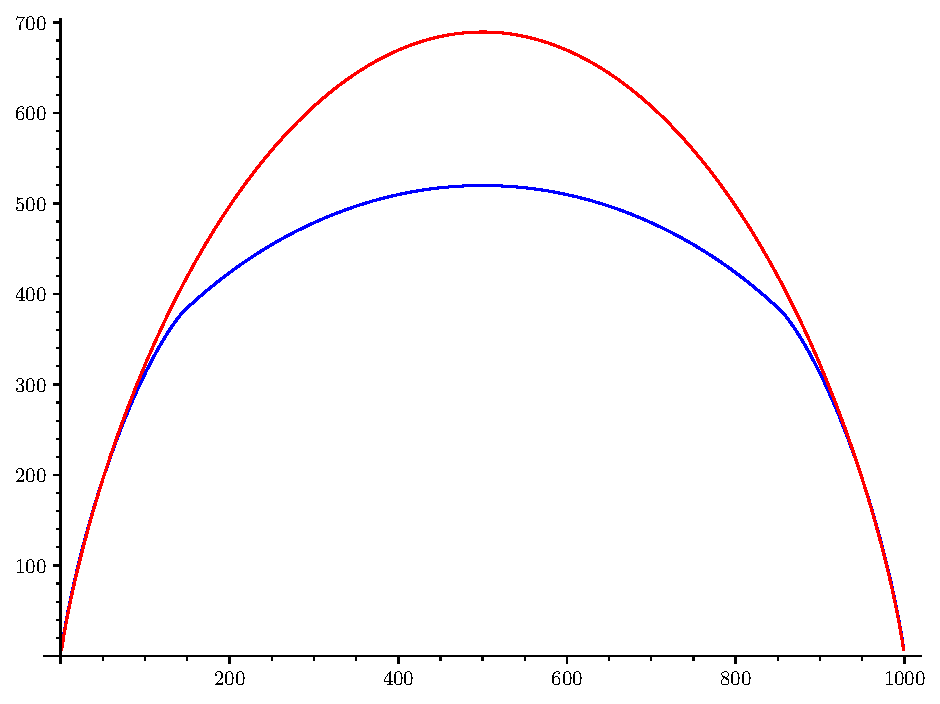
\includegraphics[width=7cm]{cauchy_estimate.pdf}
        \caption{Cauchy estimate in blue vs.\ binomial coefficients in red}
        \label{fig:cauchy_estimate}
    \end{figure}
\end{remark}
    
\begin{Prop}\label{prop:bound_sum_D_nka}
    For every $1\leq k\leq n$, fix a Boolean vector $a\ui k\in\F_2^n$. Then we have the following bound:
    \[
        \sum_{k=1}^n\left|\Dnka nk{a\ui k}\right|\leq n\cdot 2^{3n/4}.
    \]
\end{Prop}

\begin{proof}
    Simply observe that $2^{n/4}\sqrt{\frac{n^n}{(n-k)^{n-k}\cdot k^k}}$ is maximal for $k=n/2$, in which case the expression reduces to $2^{3n/4}$.
\end{proof}

\subsection{Bounding the Walsh transform of $f$}

From Property \ref{prop:bound_sum_D_nka}, we can in particular deduce that $|\wt f(a)|\leq n\cdot 2^{3n/4}+1$ for every Boolean vector $a\in\F_2^n$. This is a very pessimistic bound. In this section, we will discuss how a tighter bound on $|\wt f(a)|$ can be obtained in polynomial time in $n$.

This method is based on the identity (\ref{eqn:walsh_from_D}). For this, consider a vector $b\in\mathbb F_2^n$; we write $(p,q,r)=(p(b),q(b),r(b))$. Also, for $1\leq k\leq n$, let $b_k=b+\pi(e_k)$ and $(p_k,q_k,r_k)=(p(b_k),q(b_k),r(b_k))$. Observe that for every $1\leq k\leq n$, we have $(p_k,q_k,r_k)\in\{(p\pm1,q,r\mp 1),(p,q\pm 1,r\mp 1)\}$. Furthermore, observe that if $k\leq n/2$ and $(p_k,q_k,r_k)=(p+\alpha,q+\beta,r+\gamma)$ for $\{\alpha,\beta,\gamma\}=\{0,\pm 1\}$ with $\gamma\neq 0$, then we have $(p_{k+n/2},q_{k+n/2},r_{k+n/2})=(p+\alpha',q+\beta',r+\gamma')$ for some $\{\alpha',\beta',\gamma'\}=\{0,\pm 1\}$ with $\gamma'\neq 0$ which only depend on $\alpha$, $\beta$ and $\gamma$. Explicitly, we have $(\alpha',\beta',\gamma')=(\alpha,\beta,\gamma)$ if $\gamma=1$ and $(\alpha',\beta',\gamma')=(\beta,\alpha,\gamma)$ if $\gamma=-1$.

In the following discussion, we outline a method to determine an upper bound on $\max_{a\in\F_2^n}\wt f(a)$. A similar approach can be applied to find a lower bound on $\min_{a\in\F_2^n}\wt f(a)$, and by utilizing both, we can also obtain an upper bound on $\max_{a\in\F_2^n}|\wt f(a)|$ by making use of the following identity:
\[
    \max_{a\in\F_2^n}|\wt f(a)|=\max\Big(\max_{a\in\F_2^n}\wt f(a),-\min_{a\in\F_2^n}\wt f(a)\Big).
\]
For each $1\leq k\leq n/2$, select $\{\alpha_k,\beta_k,\gamma_k\}=\{0,\pm 1\}$ with $\gamma_k\neq 0$ such that the following expression is defined and maximized:
\[
    B_k^{p,q,r}=\mathsf D_{n,k}^{p+\alpha_k,q+\beta_k,r+\gamma_k}+\mathsf D_{n,k+n/2}^{p+\alpha_k',q+\beta_k',r+\gamma_k'}.
\]
This implies that $\Dnka{n}{k}{b_k}+\Dnka{n}{k+n/2}{b_{k+n/2}}\leq B_k^{p,q,r}$ for every $1\leq k\leq n/2$, leading to the conclusion that $\sum_{k=1}^n\Dnka nk{b_k}\leq\sum_{k=1}^{n/2} B_k^{p,q,r}$. As a result, we derive the following upper bound:
\begin{equation}\label{eqn:bound_walsh}
\max_{a\in\F_2^n}\wt f(a)\leq\max_{p+q+r=n/2}\sum_{k=1}^{n/2} B_k^{p,q,r}.
\end{equation}
Under the assumption that the values of $\mathsf{D}_{n,k}^{p,q,r}$ have already been computed for all triplets $(p,q,r)$ satisfying $p+q+r=n/2$, the bound in equation (\ref{eqn:bound_walsh}) can be determined with a computational complexity of $\mathcal{O}(n^3)$. This is because there are $\mathcal{O}(n^2)$ possible triplets $(p,q,r)$ that meet the condition $p+q+r=n/2$, and the summation itself can be computed in $\mathcal{O}(n)$.

Consider now the complexity involved in computing the values of $\mathsf{D}_{n,k}^{p,q,r}$ for all $0 \leq k \leq n$ and for all triplets $(p,q,r)$ where $p+q+r=n/2$. We claim that this computation has a complexity of $\mathcal{O}(n^3 \log n)$. Towards this, according to Property \ref{prop:generating_fct}, it is sufficient to expand the polynomials $(-z^2 + 2z + 1)^p \cdot (-z^2 - 2z + 1)^q \cdot (z^2 + 1)^r$ for all triplets $(p,q,r)$ such that $p+q+r=n/2$.

To achieve this, we first precompute the expanded polynomials $(-z^2 + 2z + 1)^p$ for each $1 \leq p \leq n/2$. This can be done recursively using the formula $(-z^2 + 2z + 1)^{p+1} = (-z^2 + 2z + 1) \cdot (-z^2 + 2z + 1)^p$. For each $p$, we need to compute the product of two expanded polynomials of degree at most $n/2$, which requires $\mathcal{O}(n \log n)$ computations . Performing this for every $p$ results in a total complexity of $\mathcal{O}(n^2 \log n)$. The same approach is used to expand the polynomials $(-z^2 - 2z + 1)^q$ and $(z^2 + 1)^r$, resulting in an overall complexity of $\mathcal{O}(n^2 \log n)$ for this precomputational step.

Finally, for each triplet $(p,q,r)$ where $p+q+r=n/2$, we multiply the expanded polynomials $(-z^2 + 2z + 1)^p$, $(-z^2 - 2z + 1)^q$, and $(z^2 + 1)^r$. These two multiplications are once more performed in $\mathcal{O}(n \log n)$. Given that there are $\mathcal{O}(n^2)$ such triplets $(p,q,r)$, the complexity of this step totals $\mathcal{O}(n^3 \log n)$. Therefore, this final step is the primary computational bottleneck, making the overall complexity of the procedure also $\mathcal{O}(n^3 \log n)$.

Table \ref{table:max_walsh_vs_bound} compares $\max_{a\in\mathbb F_2^n}|\wt f(a)|$ to the upper bound $B_n$ we find using the above method. Table \ref{table:walsh_bounds} gives all values of this bound $B_n$ for all even $1\leq n\leq 80$. As we can see from Figure \ref{fig:walsh_bound}, our bound $B_n$ is exponential in $n$.

\begin{table}
    \centering
    \begin{tabular}{|c|c|c|}
    \hline
    $n$ & $\max_{a\in\F_2^n}|W_f(a)|$ & $B_n$ \\ \hline
    $2$  & $2$     & $4$     \\
    $4$  & $8$     & $14$     \\
    $6$  & $20$    & $36$    \\
    $8$  & $52$    & $114$    \\
    $10$ & $108$   & $288$   \\
    $12$ & $292$   & $820$   \\
    $14$ & $700$   & $2\,316$  \\
    $16$ & $2\,176$  & $6\,006$  \\
    $18$ & $4\,964$  & $18\,192$  \\
    $20$ & $14\,968$ & $48\,480$ \\
    $22$ & $34\,232$ & $140\,392$ \\
    $24$ & $109\,648$ & $392\,168$ \\ \hline
    \end{tabular}
    \caption{The actual $\max_{a\in\F_2^n}|W_f(a)|$ vs.\ our bound $B_n$}
    \label{table:max_walsh_vs_bound}
\end{table}




\pmnote{@Tim, could you do a (summary) graph with the bound it gives for the nonlinearity? (Definition from the Walsh transform in the preliminaries)

Could you add curves for the majority function, $n$ even $\NL=2^{n-1}- 1/2 \binom{n}{n/2}$ , and HWBF  $n$ even $\NL=2^{n-1}- 2 \binom{n-2}{(n-2)/2}$ \cite{DAM:WCST14} Theorem 3.



}









Here is the updated table with the new values for \( B_n \) corresponding to each \( n \):

\begin{table}
    \centering
    \begin{minipage}{0.24\textwidth}
        \centering
        \begin{tabular}{|c|c|}
            \hline
            $n$ & $B_n$ \\
            \hline
            $2$  & $4.00 \cdot 10^{0}$  \\
            $4$  & $1.40 \cdot 10^{1}$  \\
            $6$  & $3.60 \cdot 10^{1}$  \\
            $8$  & $1.14 \cdot 10^{2}$  \\
            $10$ & $2.88 \cdot 10^{2}$  \\
            $12$ & $8.20 \cdot 10^{2}$  \\
            $14$ & $2.32 \cdot 10^{3}$  \\
            $16$ & $6.01 \cdot 10^{3}$  \\
            $18$ & $1.82 \cdot 10^{4}$  \\
            $20$ & $4.85 \cdot 10^{4}$  \\
            \hline
        \end{tabular}
    \end{minipage}%
    \begin{minipage}{0.24\textwidth}
        \centering
        \begin{tabular}{|c|c|}
            \hline
            $n$ & $B_n$ \\
            \hline
            $22$ & $1.40 \cdot 10^{5}$  \\
            $24$ & $3.92 \cdot 10^{5}$  \\
            $26$ & $1.14 \cdot 10^{6}$  \\
            $28$ & $3.12 \cdot 10^{6}$  \\
            $30$ & $8.90 \cdot 10^{6}$  \\
            $32$ & $2.50 \cdot 10^{7}$  \\
            $34$ & $7.14 \cdot 10^{7}$  \\
            $36$ & $2.04 \cdot 10^{8}$  \\
            $38$ & $5.75 \cdot 10^{8}$  \\
            $40$ & $1.62 \cdot 10^{9}$  \\
            \hline
        \end{tabular}
    \end{minipage}%
    \begin{minipage}{0.24\textwidth}
        \centering
        \begin{tabular}{|c|c|}
            \hline
            $n$ & $B_n$ \\
            \hline
            $42$ & $4.59 \cdot 10^{9}$  \\
            $44$ & $1.29 \cdot 10^{10}$ \\
            $46$ & $3.63 \cdot 10^{10}$ \\
            $48$ & $1.02 \cdot 10^{11}$ \\
            $50$ & $2.88 \cdot 10^{11}$ \\
            $52$ & $8.06 \cdot 10^{11}$ \\
            $54$ & $2.30 \cdot 10^{12}$ \\
            $56$ & $6.45 \cdot 10^{12}$ \\
            $58$ & $1.83 \cdot 10^{13}$ \\
            $60$ & $5.14 \cdot 10^{13}$ \\
            \hline
        \end{tabular}
    \end{minipage}%
    \begin{minipage}{0.24\textwidth}
        \centering
        \begin{tabular}{|c|c|}
            \hline
            $n$ & $B_n$ \\
            \hline
            $62$ & $1.47 \cdot 10^{14}$ \\
            $64$ & $4.09 \cdot 10^{14}$ \\
            $66$ & $1.17 \cdot 10^{15}$ \\
            $68$ & $3.25 \cdot 10^{15}$ \\
            $70$ & $9.34 \cdot 10^{15}$ \\
            $72$ & $2.60 \cdot 10^{16}$ \\
            $74$ & $7.44 \cdot 10^{16}$ \\
            $76$ & $2.08 \cdot 10^{17}$ \\
            $78$ & $5.97 \cdot 10^{17}$ \\
            $80$ & $1.65 \cdot 10^{18}$ \\
            \hline
        \end{tabular}
    \end{minipage}
    \caption{Values of $B_n$ for various $n$}
    \label{table:walsh_bounds}
\end{table}

\begin{figure}
    \centering
    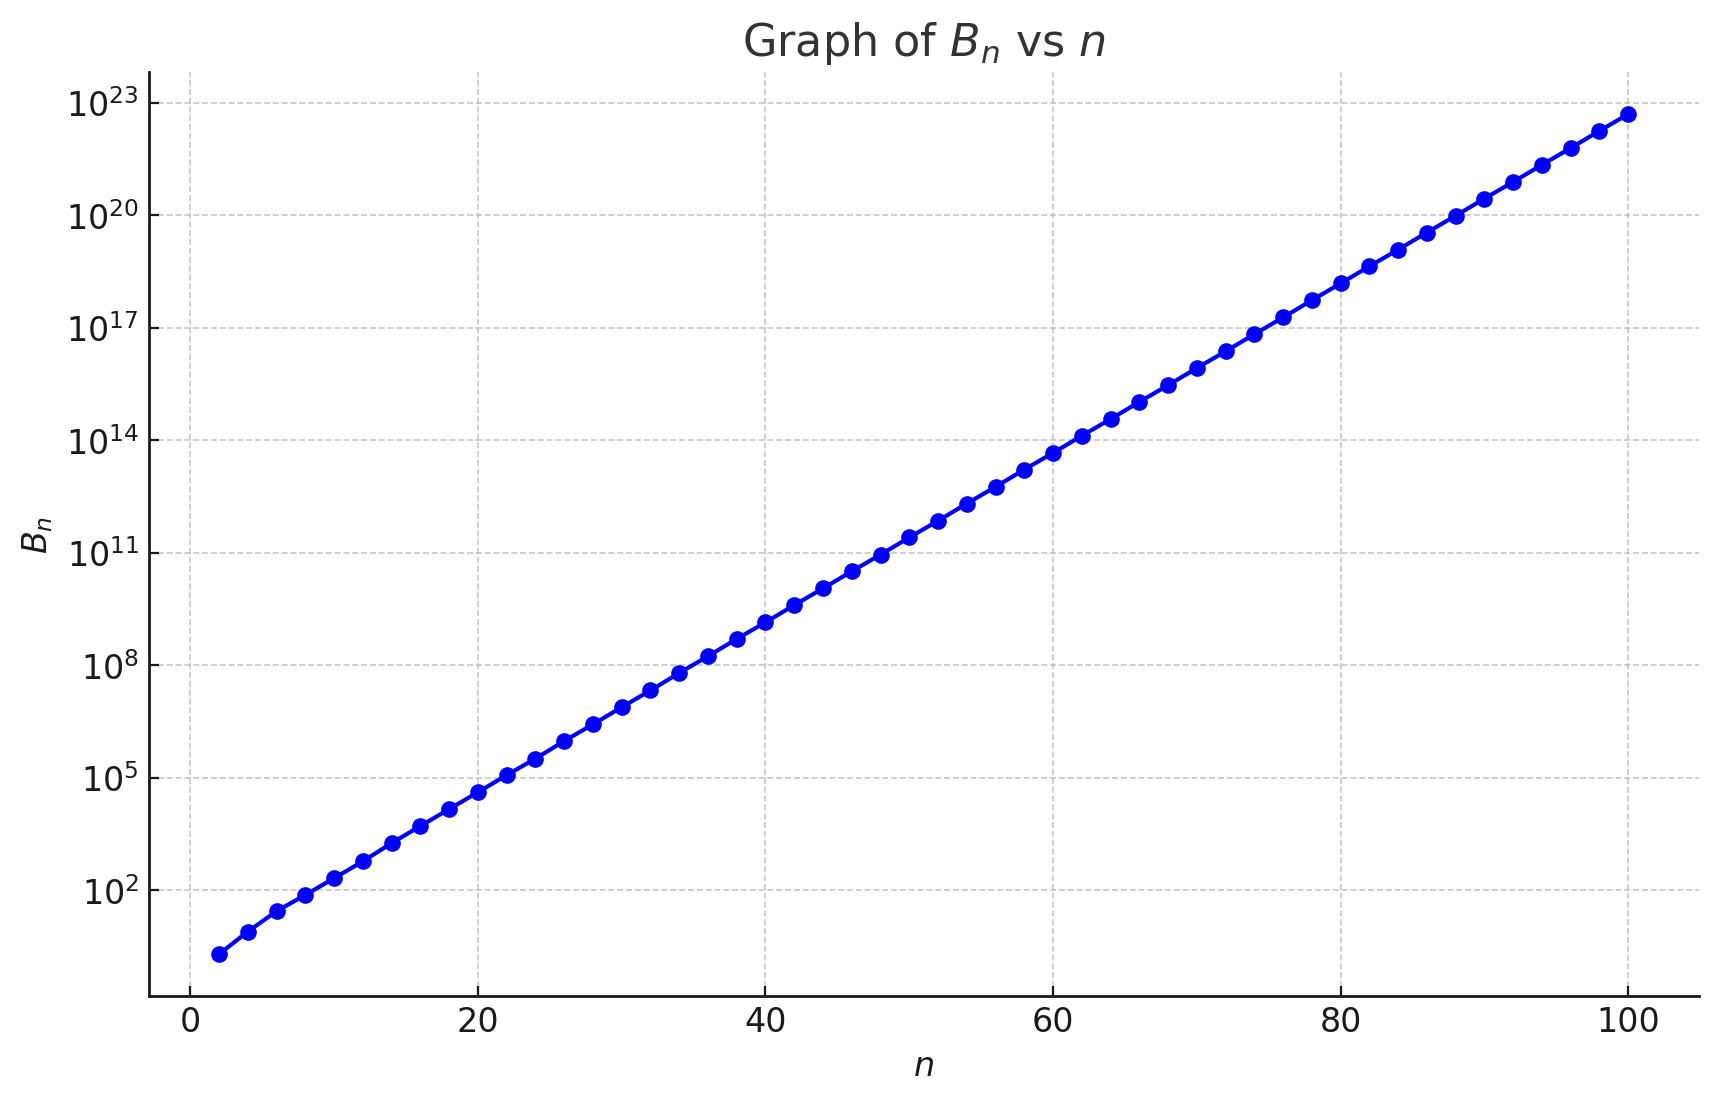
\includegraphics[width=10cm]{walsh_bound}
    \caption{Our bounds $B_n$ in terms of $n$, on a logarithmic scale}
    \label{fig:walsh_bound}
\end{figure}






\subsection{Generalization}

\begin{definition}
	Let $n\in \N$ be an even number and $t \in \N $ no greater than $n/2$, we denote by $d_{t,n}$ the function given by: $d_{t,n}(x)=\sum_{i=1}^t x_{2i-1} x_{2i}$.
	
	%	by $\Dnka{n}{k}{a}$:
	%	\[\Dnka{n}{k}{a}= \sum_{x\in \Ekn{k}{n}} (-1)^{d_n(x) +a x}\]
\end{definition}

In particular, $d_{n,n}(x)=d_n(x)$. 

We focus on the Walsh spectrum restricted to the slices of any function $d_{t,n}$

\begin{proposition}\label{prop:dtn}
	Let $t, n\in \N$ with $n$ even and $t\le n/2$, the following holds on $d_{t,n}$ for all $k\in [0,n]$:
	\[\wtk{d_{t,n}}{k}(a)=\sum_{\ell=0}^{2t} \Dnka{2t}{\ell}{b} \kraw{k-\ell}{\w(c)}{n-2t},\]
	where $b$ denotes the first $2t$ elements of $a$ and $c$ the last $n-2t$ elements.
	
	
	
	
	
\end{proposition}
\begin{proof}
	We rewrite the restricted Walsh transform, denoting $x\in \F_2^n$ by $(y,z)$ where $y\in \F_2^{2t}$ and $z \in \F_2^{n-2t}$, and similarly denoting $a$ by $(b,c)$:
	
	\begin{align*}
	\wtk{d_{t,n}}{k}(a)&=\sum_{x \in \Ekn{k}{n}} (-1)^{d_{t,n}(x)+ax}=\sum_{x \in \Ekn{k}{n}} (-1)^{d_{t,t}(y)+by +cz}\\
	&=\sum_{\ell=0}^{2t} \sum_{y \in \Ekn{\ell}{2t} \atop z \in \Ekn{k-\ell}{n-2t}} (-1)^{d_{t,t}(y)+by +cz}\\
	&=\sum_{\ell=0}^{2t} \sum_{y \in \Ekn{\ell}{2t}} (-1)^{d_{t,t}(y)+by} \left( \sum_{z \in \Ekn{k-\ell}{n-2t}} (-1)^{cz}\right)\\
	&=\sum_{\ell=0}^{2t} \Dnka{2t}{\ell}{b} \kraw{k-\ell}{\w(c)}{n-2t}.
	\end{align*}	
	
	
\end{proof}




\subsection{Algebraic immunity of $f$}

\begin{proposition}[Algebraic immunity of $f$]
	Let $n\in \N$ be even, $f$ defined as
	$f(x_1,\cdots,x_n)=\left(\sum_{i=1}^{n/2} (x_i+1) x_{i+\frac{n}{2}}\right) + \sum_{k=1}^n \phikn{k}{n} x_k$ and $h$ denote the $n$-variable HWBF, the following holds:
	\[\AI(f)\ge \AI(h)-2.\]
\end{proposition}
\begin{proof}
	Let denote by $q$ the quadratic function $\sum_{i=1}^{n/2} (x_i+1) x_{i+\frac{n}{2}}$, it allows to write $h=f+q$. 
	Let $g\neq 0$ be an annihilator of $f+ \varepsilon$ of minimum degree (where $\varepsilon \in \{0,1\}$), then the following holds:
	\[g (1+q) (h+\varepsilon) = g(1+q) (f+\varepsilon + q)=0, \]
	hence $g (1+q)$ is an annihilator of $h+ \varepsilon$. 
	If $g (1+q)\ne 0$ then $\degg(g(1+q)) \le \degg(g)+2$ and we obtain $\degg(g)\ge \AI(h) -2$. 
	Otherwise, $g (1+q)= 0$ implies that $g$ annihilates $1+q$ and therefore $0=g (f+\varepsilon + 1 +q)=g(h+ \varepsilon +1)$ that is $\degg(g)\ge \AI(h)$. 
	Summarizing, for any non null annihilator $g$ of $f$ or $f+1$ we get $\degg(g)\ge \AI(h)-2$, it allows to conclude $\AI(f)\ge \AI(h)-2$.
	
\end{proof}

From~\cite{DAM:WCST14} Theorem 4, the algebraic immunity of the HWBF is at least $\lfloor n/3\rfloor +1$, which leads to $\lfloor n/3\rfloor -1$ for $f$.



\newpage

%%%%%%%%%%%%%%%%%%%%%%%%%%%%%%%%%%%%%%%


\ifnum\full=0
%%%%%%%%%%%%%%%%%%%%%%%%%%%%%%%%%%%%%%%%%%%%
\bibliographystyle{splncs04}
\bibliography{add}
%%%%%%%%%%%%%%%%%%%%%%%%%%%%%%%%%%%%%%%%%%%%
\else
%%%%%%%%%%%%%%%%%%%%%%%%%%%%%%%%%%%%%%%%%%%%
\bibliographystyle{alpha}
\bibliography{add}
%%%%%%%%%%%%%%%%%%%%%%%%%%%%%%%%%%%%%%%%%%%%
\fi

\end{document}
